\documentclass[main.tex]{subfiles}

\begin{document}

\section{Chapter 1}

\hrulefill

Jan 27, 2017

\vspace{3mm}

\subsection{Conservation Law}

Want to describe density of a medium at some time.

In one dimension, imagine a tube with uniform cross sectional area $A$ abstracted as a line.

\begin{figure}[ht]
        \centering
        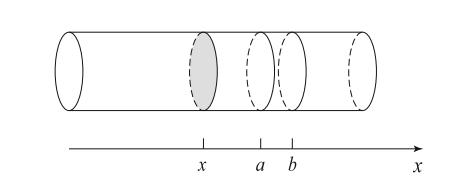
\includegraphics[width=0.5\textwidth]{conservation-tube}
        \caption{A tube with some quantity of interest having density $u$.}
        \label{fig:conservation-tube}
\end{figure}

Possible mediums:
\begin{itemize}
    \item Dye molecules in water
    \item Temperature
    \item Cars
\end{itemize}

Medium should be conserved excluding a \textit{source} term (no creation or destruction of matter/energy/etc.)

Consider $\phi(x, t, ...) = \textrm{rate of flux of the medium rightward through position }x\textrm{ at time t}$

Using conservation property:

\begin{align}
\frac{d}{dt} \int_a^b u(x,t)\,dx &= \textrm{ influx - outflux} \\
                                 &= \phi(a) - \phi(b)
\end{align}

Generalization with sources/sinks $f(x, t, ...)$ = rate at which something is added (+) or removed (-) from the system at position $x$ and time $t$.

With this:
\begin{align}
\frac{d}{dt} \int_a^b u(x,t)\,dx &= \textrm{ influx - outflux + source} \\
                                 &= \phi(a) - \phi(b) + \int_a^b f\,dx
\end{align}

Rewriting,

\begin{align}
\frac{d}{dt}\int_a^bu\,dx &= \int_a^b -\phi_x + f\,dx \\
\int_a^b u_t\,dx          &= \int_a^b -\phi_x + f\,dx \\
u_t &= -\phi_x + f
\end{align}

\begin{equation}
\label{eq:conservation-law}
u_t + \phi_x = f
\end{equation}

\subsection{Advection}
Advection transport: $\phi(x, t, u) = c(x, t)u(x, t)$
\begin{itemize}
    \item $c(x, t)$ is a speed
    \item $u(x, t)$ is a density
\end{itemize}

Assume $c$ is a constant and there is no source:

\begin{equation}
\label{eq:advection}
u_t + cu_x = 0
\end{equation}

Put $u_t$ and $u_x$ into vector

$\implies (c, 1) \cdot (u_x, u_t) = 0$

This means that the directional derivative of $u$ in the direction $(c, 1)$ is 0.

Therefore, $u$ is constant along lines $x(t) = x_0 + ct$

For example, $u(x_0+ct, t) = u_0(x_0)$.

Therefore, $u(x, t) = u_0(x-ct)$

\subsection{Diffusion}

Diffusion: $\phi = -ku_x$, $k > 0$ (Fick's law of diffusion or Fourier's Law of heat conduction).

This implies that $u$ with positive slope yields leftward flux and $u$ with negative slope yields rightward flux.

Plugging in, $u_t = -(-ku_x)_x = ku_{xx}$

\begin{equation}
u_t - ku_{xx} = 0
\end{equation}

We can combine (\ref{eq:advection}) and (\ref{eq:heat}): $\phi = cu - ku_x$

This yields the advection-diffusion equation
\begin{equation}
    \label{eq:advection-diffusion}
    u_t + cu_x - ku_{xx} = f
\end{equation}

Example: with advection-diffusion, $t\ge0$, $x\in\mathbb{R}$ or $x\in[0, l]$

\end{document}
